\begin{figure}[ht!]  % 'htbp' suggests placement options
    \centering
    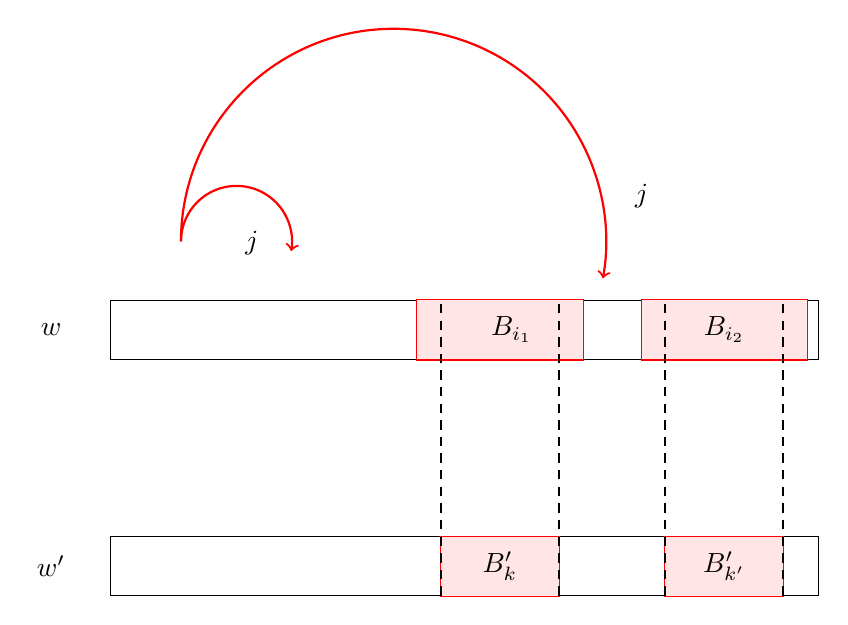
\begin{tikzpicture}[scale=1.5]
        % Main Rectangle w
        \draw (0,0) rectangle (6,0.5);
        \node at (-0.5, 0.25) {\(w\)};

        % Smaller Rectangle 1 - Border color red
        \draw[draw=red, thick] (4.5,0) rectangle (5.9,0.5);
        \fill[red!10] (4.5,0) rectangle (5.9,0.5);
        \node at (5.2,0.25) {$B_{i_2}$};

                
        \draw[draw=red, thick] (2.6,0) rectangle (4.0,0.5);
        \fill[red!10] (2.6,0) rectangle (4.0,0.5);
        \node at (3.4,0.25) {$B_{i_1}$};
        
%%%%%%%%%%%%%%%%%%%%%%%%%%%%%%%%%%%%%%%%%%%%%%%%%%%%%%%%%%%%%%%%%%%%%%

        \draw (0,-1.5) rectangle (6,-2.0);
        \node at (-0.5, -1.75) {\(w'\)};

        \draw[draw=red, thick] (4.7,-2) rectangle (5.7,-1.5);
        \fill[red!10] (4.7,-2.0) rectangle (5.7,-1.5);
        \node at (5.2,-1.75) {$B'_{k'}$};
        \draw[draw=black, thick, dashed] (4.7,-2.0) rectangle (4.7,0.5);
        \draw[draw=black, thick, dashed] (5.7,-2.0) rectangle (5.7,0.5);
        
        \draw[draw=red, thick] (2.8,-2.0) rectangle (3.8,-1.5);
        \fill[red!10] (2.8,-2.0) rectangle (3.8,-1.5);
        \node at (3.3,-1.75) {$B'_{k}$};
        \draw[draw=black, thick, dashed] (2.8,-2.0) rectangle (2.8,0.5);
        \draw[draw=black, thick, dashed] (3.8,-2.0) rectangle (3.8,0.5);

                % Semicircular arrow
        \draw[->, thick, red] (0.6,1.0) arc[start angle=180, end angle=-10, radius=1.8cm];
        \draw[->, thick, red] (0.6,1.0) arc[start angle=180, end angle=-10, radius=0.47cm];
        
        \node[align=center, above] at (4.5,1.2) {\(j\)};
        \node[align=center, above] at (1.2,0.8) {\(j\)};


    \end{tikzpicture}
    \label{fig:case_1_c_2}
\end{figure}